% \begin{itemize}
% \item component-based commissioning model
% \item control components to handle the commissioning of any existing
%   component in any language
% \item goals: programmable, composable, reusable, efficient
% \item composed of:
%   \begin{itemize}
%   \item meta-model
%   \item graphical language
%   \item concrete language
%   \item formal specification (next section)
%   \item formal operational semantics (next section)
%   \end{itemize}
% \item meta-models of assembly and components (add groups)
% \item example Apache/MariaDB with graphical and concrete syntax
% \item simplified explanation of the operational semantics (middleware)
% \item discussion on the goals
% \end{itemize}

%%%%%%%%%%%%%%%%%%%%%%%%%%
\subsection{Principles}

\mad is a component-based coordination model for commissioning
procedures. Usually, component models are used to write
distributed software in a modular fashion while having guarantees on
its composition, thus improving separation of concerns between
developers, easing the way for re-use of existing pieces of code and
enhancing flexibility and maintainability of code. \mad makes use of
these properties for the design of distributed software commissionings
instead of code design.

A \mad component is called a \emph{control} component as it is only
intended to model the commissioning procedure of an already existing
component, module or service. A \mad component is a type containing
places that represent milestones of the commissioning, and transitions
that connect the places together and represent actions to be performed
between milestones (\eg \texttt{apt-get install}, \texttt{docker pull},
etc.). If multiple transitions leave a place, their parallel execution
is automatically handled and synchronized by \mad. A component may
have dependencies towards other components. Such dependencies are declared
through a well-known object in component-based software engineering:
ports. Four types of ports, working in pairs, are available in \mad:
service-provide and service-use, data-provide and data-use ports. By
using ports, each component type can be defined independently and
component instances can be connected later by another developer, thus
improving the separation of concerns and the re-use of commissioning
procedures. A service-provide port is bound to a group of places that
represents the milestones where the service is offered. A data-provide
port is bound to a single place where a value is assigned to the
port. Finally, both use ports are bound to one or multiple transitions
where data and service requirements are actually used.

The overall commissioning procedure of a distributed software system
is built by composition in an \emph{assembly}, where component
types are instanciated and connected. All control components execute
simultaneously, thus introducing more parallelism (in addition to
parallel transitions). Intuitively, two components connected by their
respective compatible ports will automatically be coordinated so
that a component cannot use a service or data if the associated
provide port is not enabled.

\mad offers the expressivity required to design composable and parallel
commissioning procedures for complex distributed software systems.

\begin{figure}[tbp]
  \begin{center}
    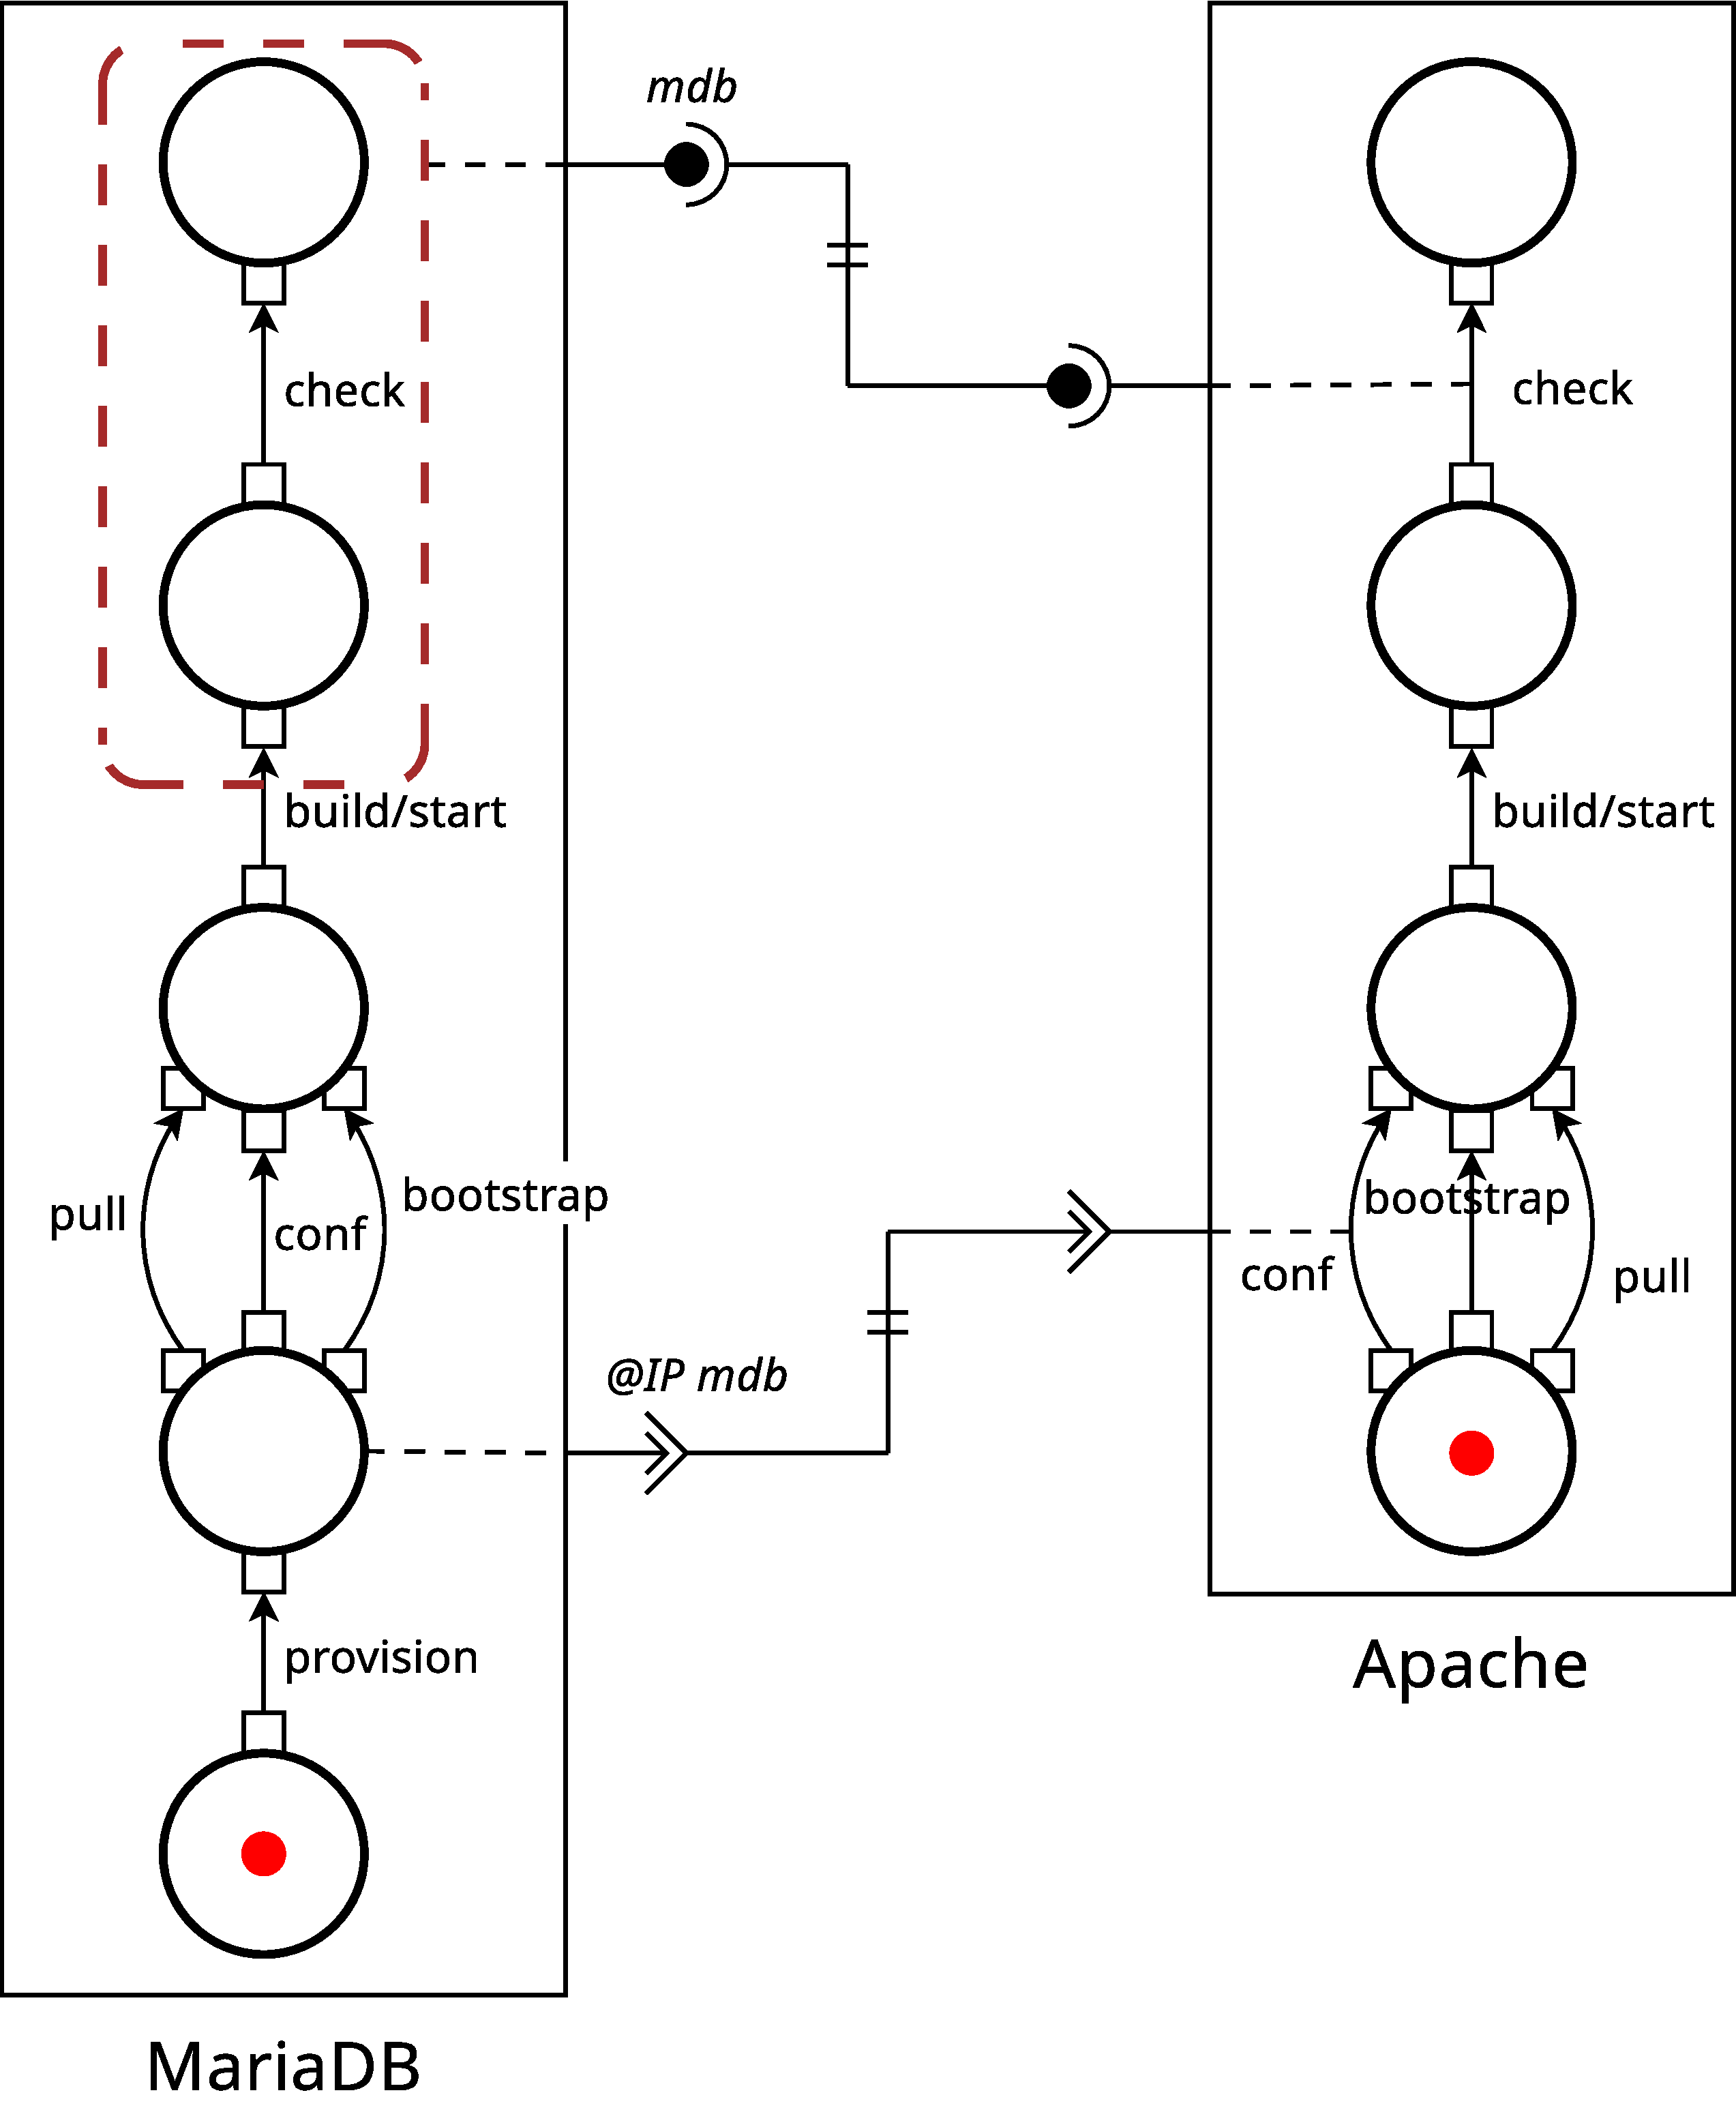
\includegraphics[width=0.7\linewidth]{./images/apachebdd.pdf}
  \end{center}
  \caption{Example of a commissioning assembly with two components
    Apache and MariaDB. Places are represented by circles, transitions
    by arrows between places, service ports by small black circles and
    semi-circles, data ports by outgoing or incoming arrows from
    components. Two initial red tokens are placed in each initial
    place of components in this example.}
  \label{fig:example}
\end{figure}

\paragraph{Example}{ Figure~\ref{fig:example} depicts the \mad
  commissioning of an Apache web server and a MariaDB database. This
  example is based on a real container-based deployment described by
  RedHat\footnote{\url{https://access.redhat.com/documentation/en-us/red_hat_enterprise_linux_atomic_host/7/html/getting_started_with_containers/install_and_deploy_an_apache_web_server_container}}%
  $^,$%
  \footnote{\url{https://access.redhat.com/documentation/en-us/red_hat_enterprise_linux_atomic_host/7/html/getting_started_with_containers/install_and_deploy_a_mariadb_container}}. Two
  \mad control components are declared in this example: Apache and
  MariaDB. Apache contains four places (white circles), or
  milestones, while MariaDB contains five places. Some parallel
  transitions are declared for each of the component and can be
  observed in the figure (parallel arrows). Both components have two
  ports. MariaDB provides both data and a service (once installed),
  while Apache uses a service and data. Figure~\ref{fig:example}
  shows the assembly of one Apache and one MariaDB instanciated from
  their component types. These instances are connected by their
  ports. Indeed, the Apache configuration depends on the IP adress of the
  MariaDB component, and the testing phase for Apache, called
  \texttt{check}, uses the MariaDB service.}

In \mad, two kinds of \emph{actors} are considered. The first is the
developer of a control component, who may be the author of the
associated existing piece of code, another developer, or even a
system operator or administrator. The second is the developer of an assembly,
typically a system operator or administrator who wants to write
the overall commissioning procedure of a distributed software system
to deploy on their infrastructure. One important benefit of \mad is
its clear separation of concerns between the commissioning of a single
component on the one hand, and the composition of an assembly, without
having to care about the detailed commissioning of each component on
the other hand. For instance, even if Ansible offers properties close
to composition (\eg roles, playbooks, tasks, etc.), the system operator
still has to determine the correct order of composition. By contrast, the
correct coordination, hence the correct order of execution, is
automatically guaranteed by the \mad semantics and the composition of
the component instances. The composition viewpoint is illustrated in
Figure~\ref{fig:simple}, where the details of each component not
needed for composition are omitted. This type of property has also been offered by
Aeolus~\cite{}, albeit without parallelism within components.

\begin{figure}[tbp]
  \begin{center}
    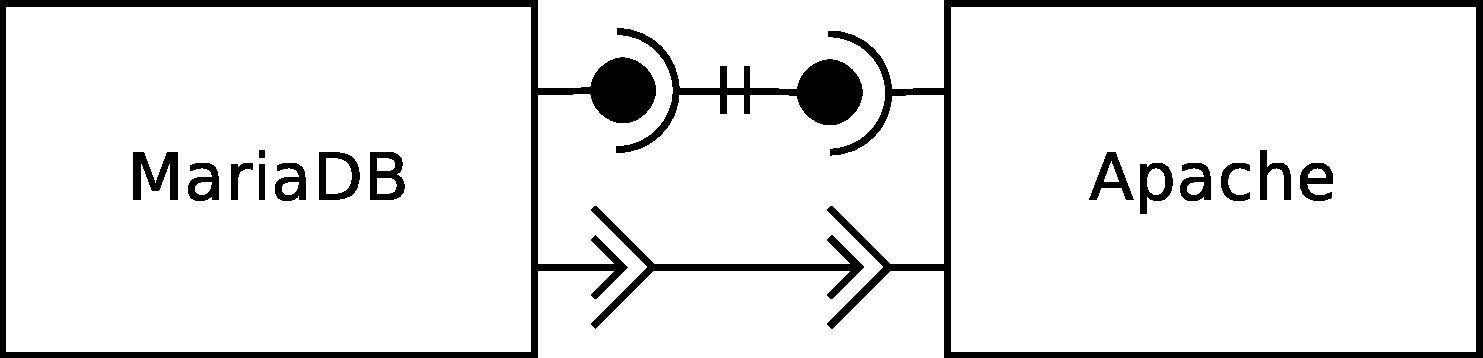
\includegraphics[width=0.6\linewidth]{./images/simpleass.pdf}
  \end{center}
  \caption{\mad assembly of an Apache component and a MariaDB
    component without knowing the details of each component.}
  \label{fig:simple}
\end{figure}

\mad is a formal component-based commissioning model that will be
detailed in Section~\ref{sec:formal_model}. \mad also comes with a
prototype and a concrete syntax.

%%%%%%%%%%%%%%%%%%%%%%%%%%
% \subsection{Meta-model}

% \HC[Maverick]{figures a refaire avec nos discussions}

\begin{figure}[tbp]
  \begin{center}
    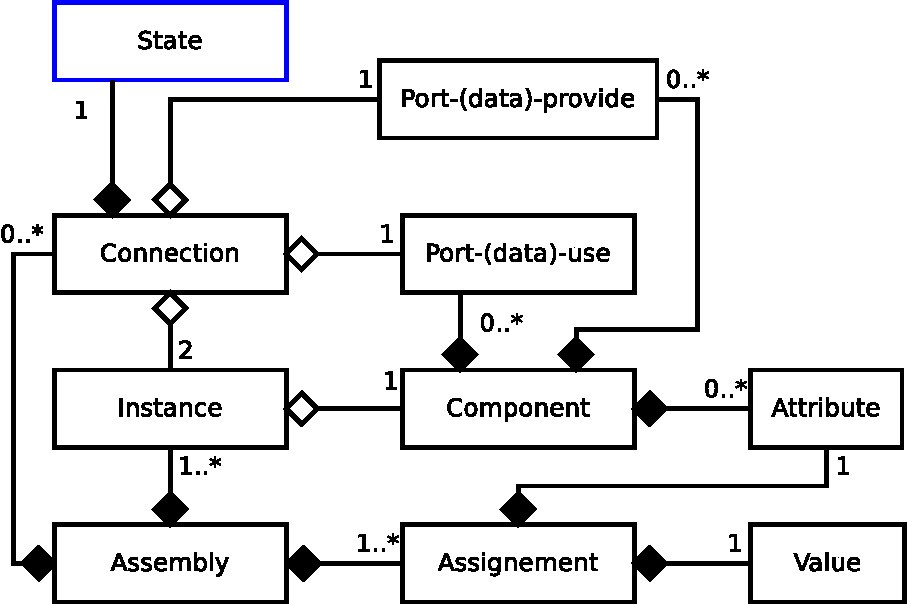
\includegraphics[width=0.9\linewidth]{./images/ass_uml.pdf}
  \end{center}
  \caption{\mad meta-model of an assembly, \ie an overall
    commissioning procedure of a distributed software.}
  \label{fig:mmass}
\end{figure}

% Figures~\ref{fig:mmass} and~\ref{fig:mmcomp} respectively depict the
% UML diagram representing the \mad meta-model of an assembly, and the
% meta-model of a component. A \mad assembly is not different from a
% usual assembly in any component model of the literature. An assembly
% basically contains component instances, connected to each other
% through their compatible ports. One specificity is that \mad handles
% four types of ports instead of usually two, by dissociating service
% ports from data ports, each having their own semantics. Intuitively,
% unlike service ports, data ports act as data registries thus, once
% activated, they will remain active forever.

\begin{figure}[tbp]
  \begin{center}
    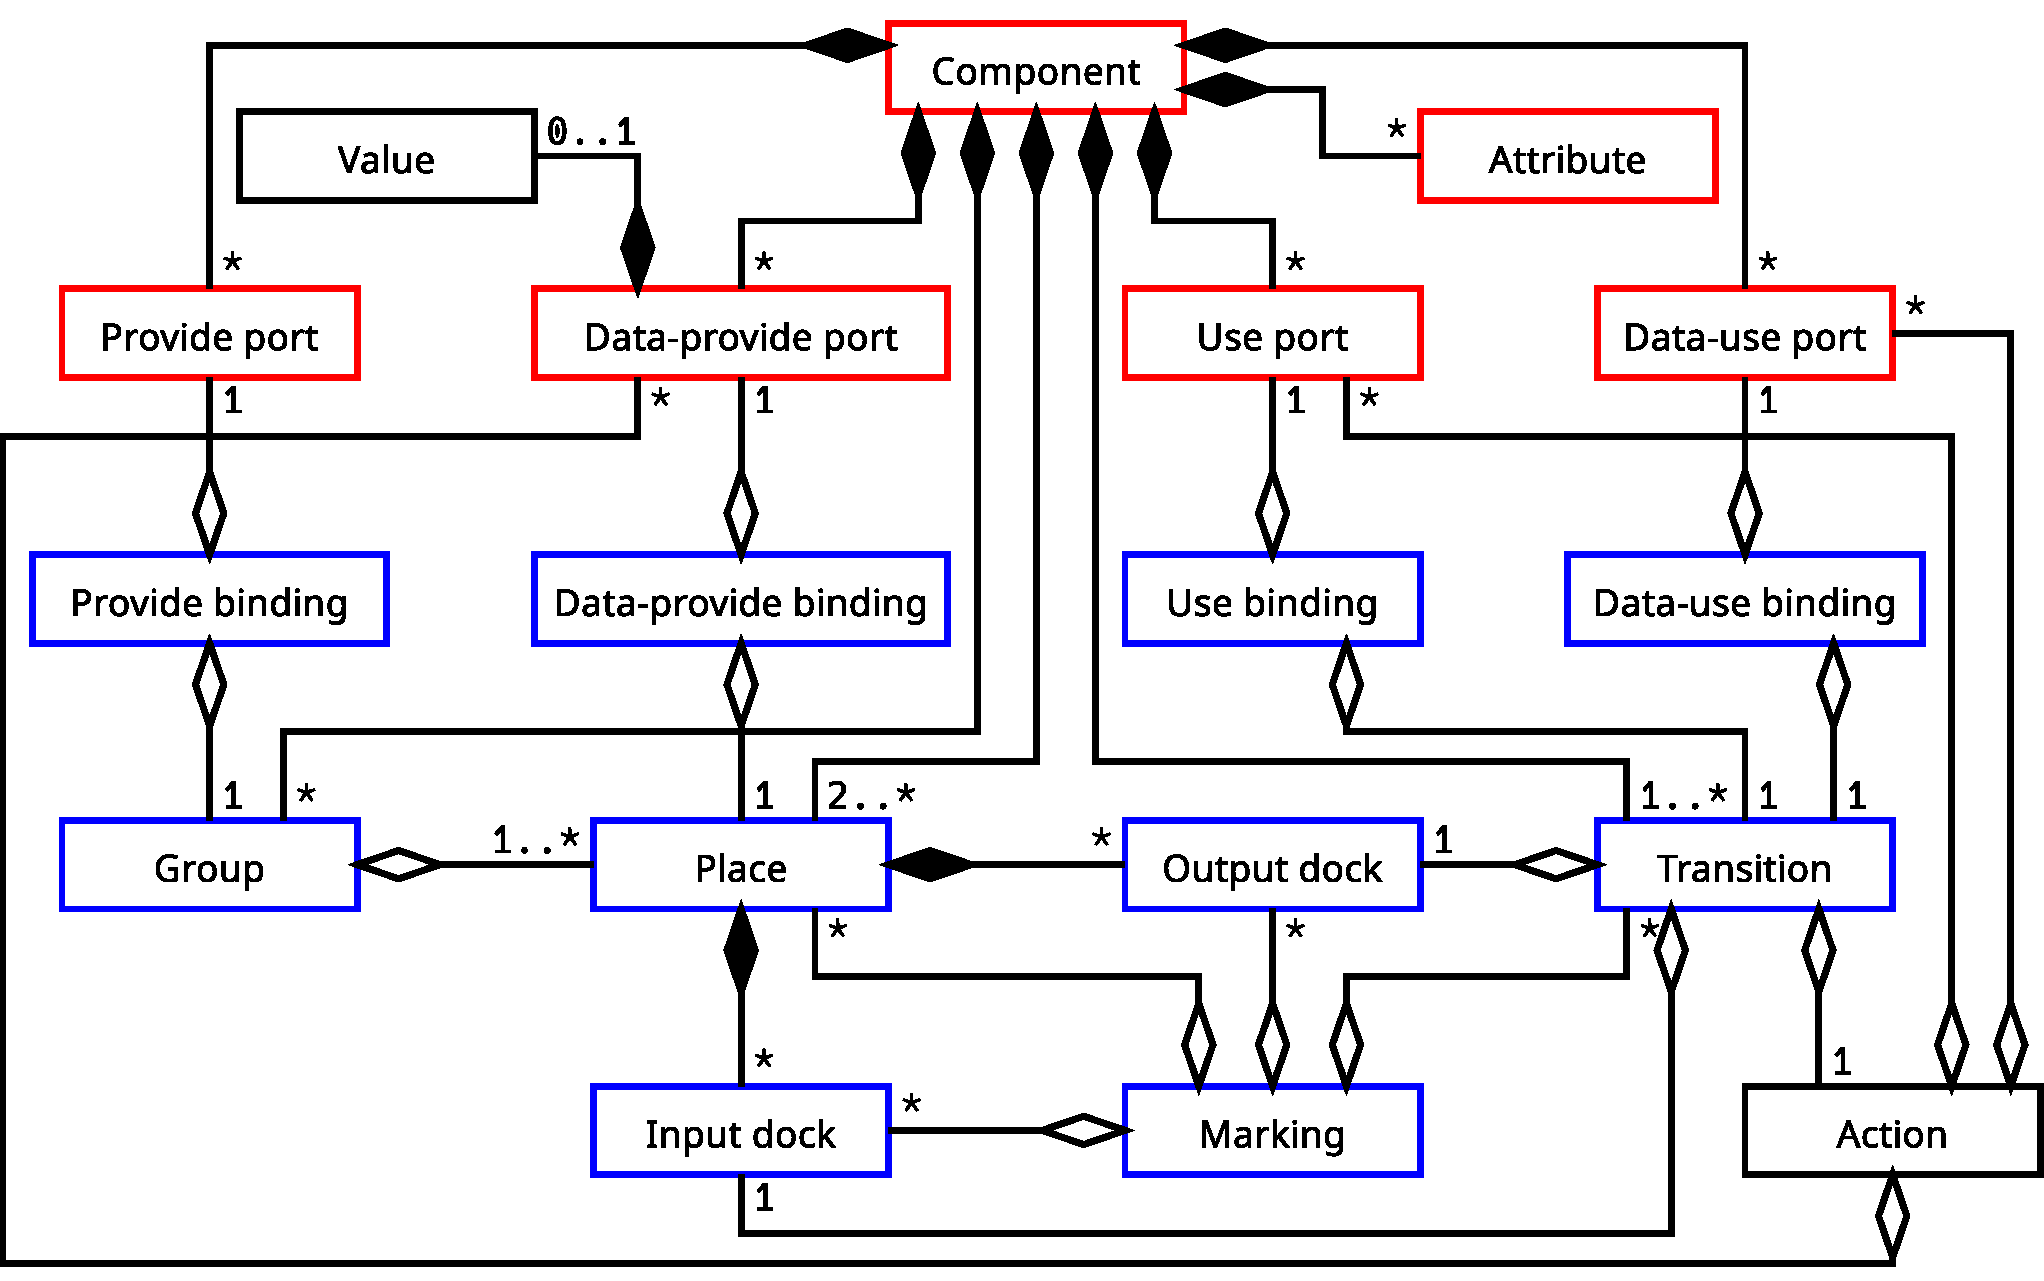
\includegraphics[width=0.9\linewidth]{./images/component_uml.pdf}
  \end{center}
  \caption{\mad meta-model of a component, \ie the commissioning
    procedure of a single component (\ie module or service).}
  \label{fig:mmcomp}
\end{figure}

% However, as already explained a \mad component is very different
% from usual components in the literature. A component type contains a
% set of places, a set of transitions, and a set of service-provide,
% service-use, data-provide and data-user ports.
% Service-provide ports (service or data) are bound to groups of
% places. Those groups of places represent the sub-part of the
% commissioning procedures where a given service is provided. A
% data-provide port is simply bound to one place from which the data is
% provided. Use ports (data or service) are bound to transitions where
% the corresponding data or services modeled by ports are actually used
% by the code executed by the transition.

%%%%%%%%%%%%%%%%%%%%%%%%%%
\subsection{Concrete language}

The concrete syntax of \mad has been implemented in Python. \mad is a
simple declarative language that follows the model previously
presented to define, first, component types, and second, assemblies of
components. Listing~\ref{codemdb} shows the declaration of the MariaDB
component type of Figure~\ref{fig:example}. Lines 3 to 8 declare
the places of the component type. A place is
identified by a unique \texttt{string}. Lines 9 to 15
declare the transitions of the component type. A transition is
identified by a unique key (a \texttt{string}), and is associated
through a dictionnary with a source and a destination place. Moreover,
each transition is associated with a function to call to perform
corresponding actions. For instance, the function \texttt{f\_pull} of
transition \texttt{pull} is declared on line 20, and provides the code
to execute during this transition. Finally lines 16 to 19 declare the
ports of the component type. A port is identified by a unique key (a
\texttt{string}), and is associated with a type and the elements to
which it is bound. As already described, service-provide ports are
bound to a group of places, data-provide ports to a single place, and
both service-use and data-use ports to a set of transitions. In the
case of MariaDB one service-provide port, namely \texttt{serv}, is
provided both at \texttt{std} and \texttt{chd} places (see the group
in Figure~\ref{fig:example}), and one data-provide port, namely
\texttt{ip} is provided from the first place \texttt{wtg}.

\begin{lstlisting}[label=codemdb,caption=Madeus code of the MariaDB
  component type.]
class MariaDB (Component):
  def create(self):
    places = [
        'wtg',
        'cfd',
        'std',
        'chd'
    ]
    transitions = {
        'pull': ('wtg', 'cfd', self.f_pull),
        'conf': ('wtg', 'cfd', self.f_conf),
        'bootstrap': ('wtg', 'cfd', self.f_boots),
        'start': ('cfd', 'std', self.f_start),
        'check': ('std', 'chd', self.f_check)
    }
    dependencies = {
        'ip': (DepType.DATA_PROVIDE, 'wtg'),
        'serv': (DepType.PROVIDE, ['std','chd'])
    }
    def f_pull(self):
        # execution of bash scripts
        # execution of ansible playbooks
        # etc.
    def f_conf(self):
        # ...
    def f_boots(self):
        # ...
    def f_start(self):
        # ...
    def f_check(self):
        # ...
\end{lstlisting}


Similarly, Listing~\ref{codeapache} shows the declaration of the
Apache component of Figure~\ref{fig:example} which has one less place
and one less transition compared to MariaDB. Furthermore, the Apache
component type contains one service-use port and one data-use port
(lines 18 to 21).

\begin{lstlisting}[label=codeapache,caption=Madeus code of the Apache
  component type.]
class Apache (Component):
  def create(self):
    places = [
        'wtg',
        'prd',
        'cfd',
        'std',
        'chd'
    ]
    transitions = {
        'provision': ('wtg','prd', self.f_prov),
        'pull': ('pr', 'cfd', self.f_pull),
        'conf': ('pr', 'cfd', self.f_conf),
        'bootstrap': ('prd', 'cfd', self.f_boots),
        'start': ('cfd', 'std', self.f_start),
        'check': ('std', 'chd', self.f_check)
    }
    dependencies = {
        'ipMDB': (DepType.DATA_USE, ['conf']),
        'serviceMDB': (DepType.USE, ['check'])
    }

    def f_prov(self):
        # execution of bash scripts
        # execution of ansible playbooks
        # etc.
    def f_pull(self):
        # ...
    def f_conf(self):
        # ...
    def f_boots(self):
        # ...
    def f_start(self):
        # ...
    def f_check(self):
        # ...
\end{lstlisting}


Finally, the Listing~\ref{codeass} shows the declaration of the
assembly of components of Figure~\ref{fig:example}. First, lines 6 and
7 respectively instanciate component types MariaDB and Apache
previously declared. Second, line 9 to 13 are as follows: the creation
of an assembly, the addition of component instances to the assembly,
the connections of the components. Finally, lines 15 and 16 run the
assembly to perform the commissioning of MariaDB/Apache. An overview
of this execution is given in the next section.

\begin{lstlisting}[label=codeass,caption=Madeus code of the assembly
  of Figure~\ref{fig:example}.]
import mariadb
import apache

if __name__ == '__main__':

  mdb = MariaDB() # Component B
  apache = Apache() # Component C

  ass = Assembly()
  ass.add('MDB', mdb)
  ass.add('Apache', apache)
  ass.connect(apache, 'ipMDB', mdb, 'ip')
  ass.connect(apache, 'servMDB', mdb, 'serv')

  mad = Mad(ass)
  mad.run()
\end{lstlisting}


%%%%%%%%%%%%%%%%%%%%%%%%%%
\subsection{Execution}

\SR{The way in which docks are introduced here is confusing}

In \mad, executing a commissioning procedure requires the execution of an
assembly. The \mad execution model is governed by operational
semantics rules to move from one configuration to another. The concept
of configuration, which is introduced formally in
Section~\ref{sec:formal_model}, intuitively corresponds to a snapshot
of the execution of an assembly, in other words the location of the
tokens and values currently associated to data-provide ports. In
practice, semantics rules move tokens from places to transitions within
components. Those rules are inspired by those of Petri nets, yet have
a specific semantics for transitions, groups and ports. Details of the
transformation from a \mad assembly to a Petri net have been given
in~\cite{coullon:hal-02323641}. The execution of a \mad assembly is
defined by four operational semantic rules. In this section, we only
sketch the role of each of these rules. They are formally specified in
Section~\ref{sec:forma_model}. Before giving the role of each rule,
one can note in Figure~\ref{fig:example} the small squares that have
not been explained yet. These squares represent \emph{docks}. Each
place has input and output transitions, and each transition has a
source dock and a destination dock. Docks have not been detailed
previously because they are automatically infered from the concrete
syntax of \mad. However, this concept is needed to explain the
execution of a \mad assembly as it is used to handle parallelism and
synchronization of transitions.
%
\begin{enumerate}
\item \emph{Firing a transition}: when the source dock of a transition
  contains a token and when all use ports of a transition have their
  associated connections activated, the token is moved from the source
  dock to the transition, which is not considered atomic as it is
  associated with an action function.
\item \emph{Ending a transition}: when a transition holds a token and
  when the action associated to the transition is terminated, the
  token is moved from the transition to its destination dock.
\item \emph{Entering a place}: when all input docks associated to a
  place hold a token, those tokens can be merged to a single one, located
  within the place.
\item \emph{Leaving a place}: when a place holds a token, and if the
  token leaving that place does not cause a provide port currently
  used by other components to be disabled,
  the token can be duplicated and placed in each output dock of the
  place.
\end{enumerate}

One can note that a data connection cannot be disabled. It
indefinitely holds the last data value.
%\CP[HC]{Correct?}
%\HC{je n'ai pas parlé des groupes pour simplifier le discours. je ne pense pas en parler car ce n'est pas utile dans les exemples.}
%\CP{ok}

\begin{figure}[tbp]
  \begin{center}
    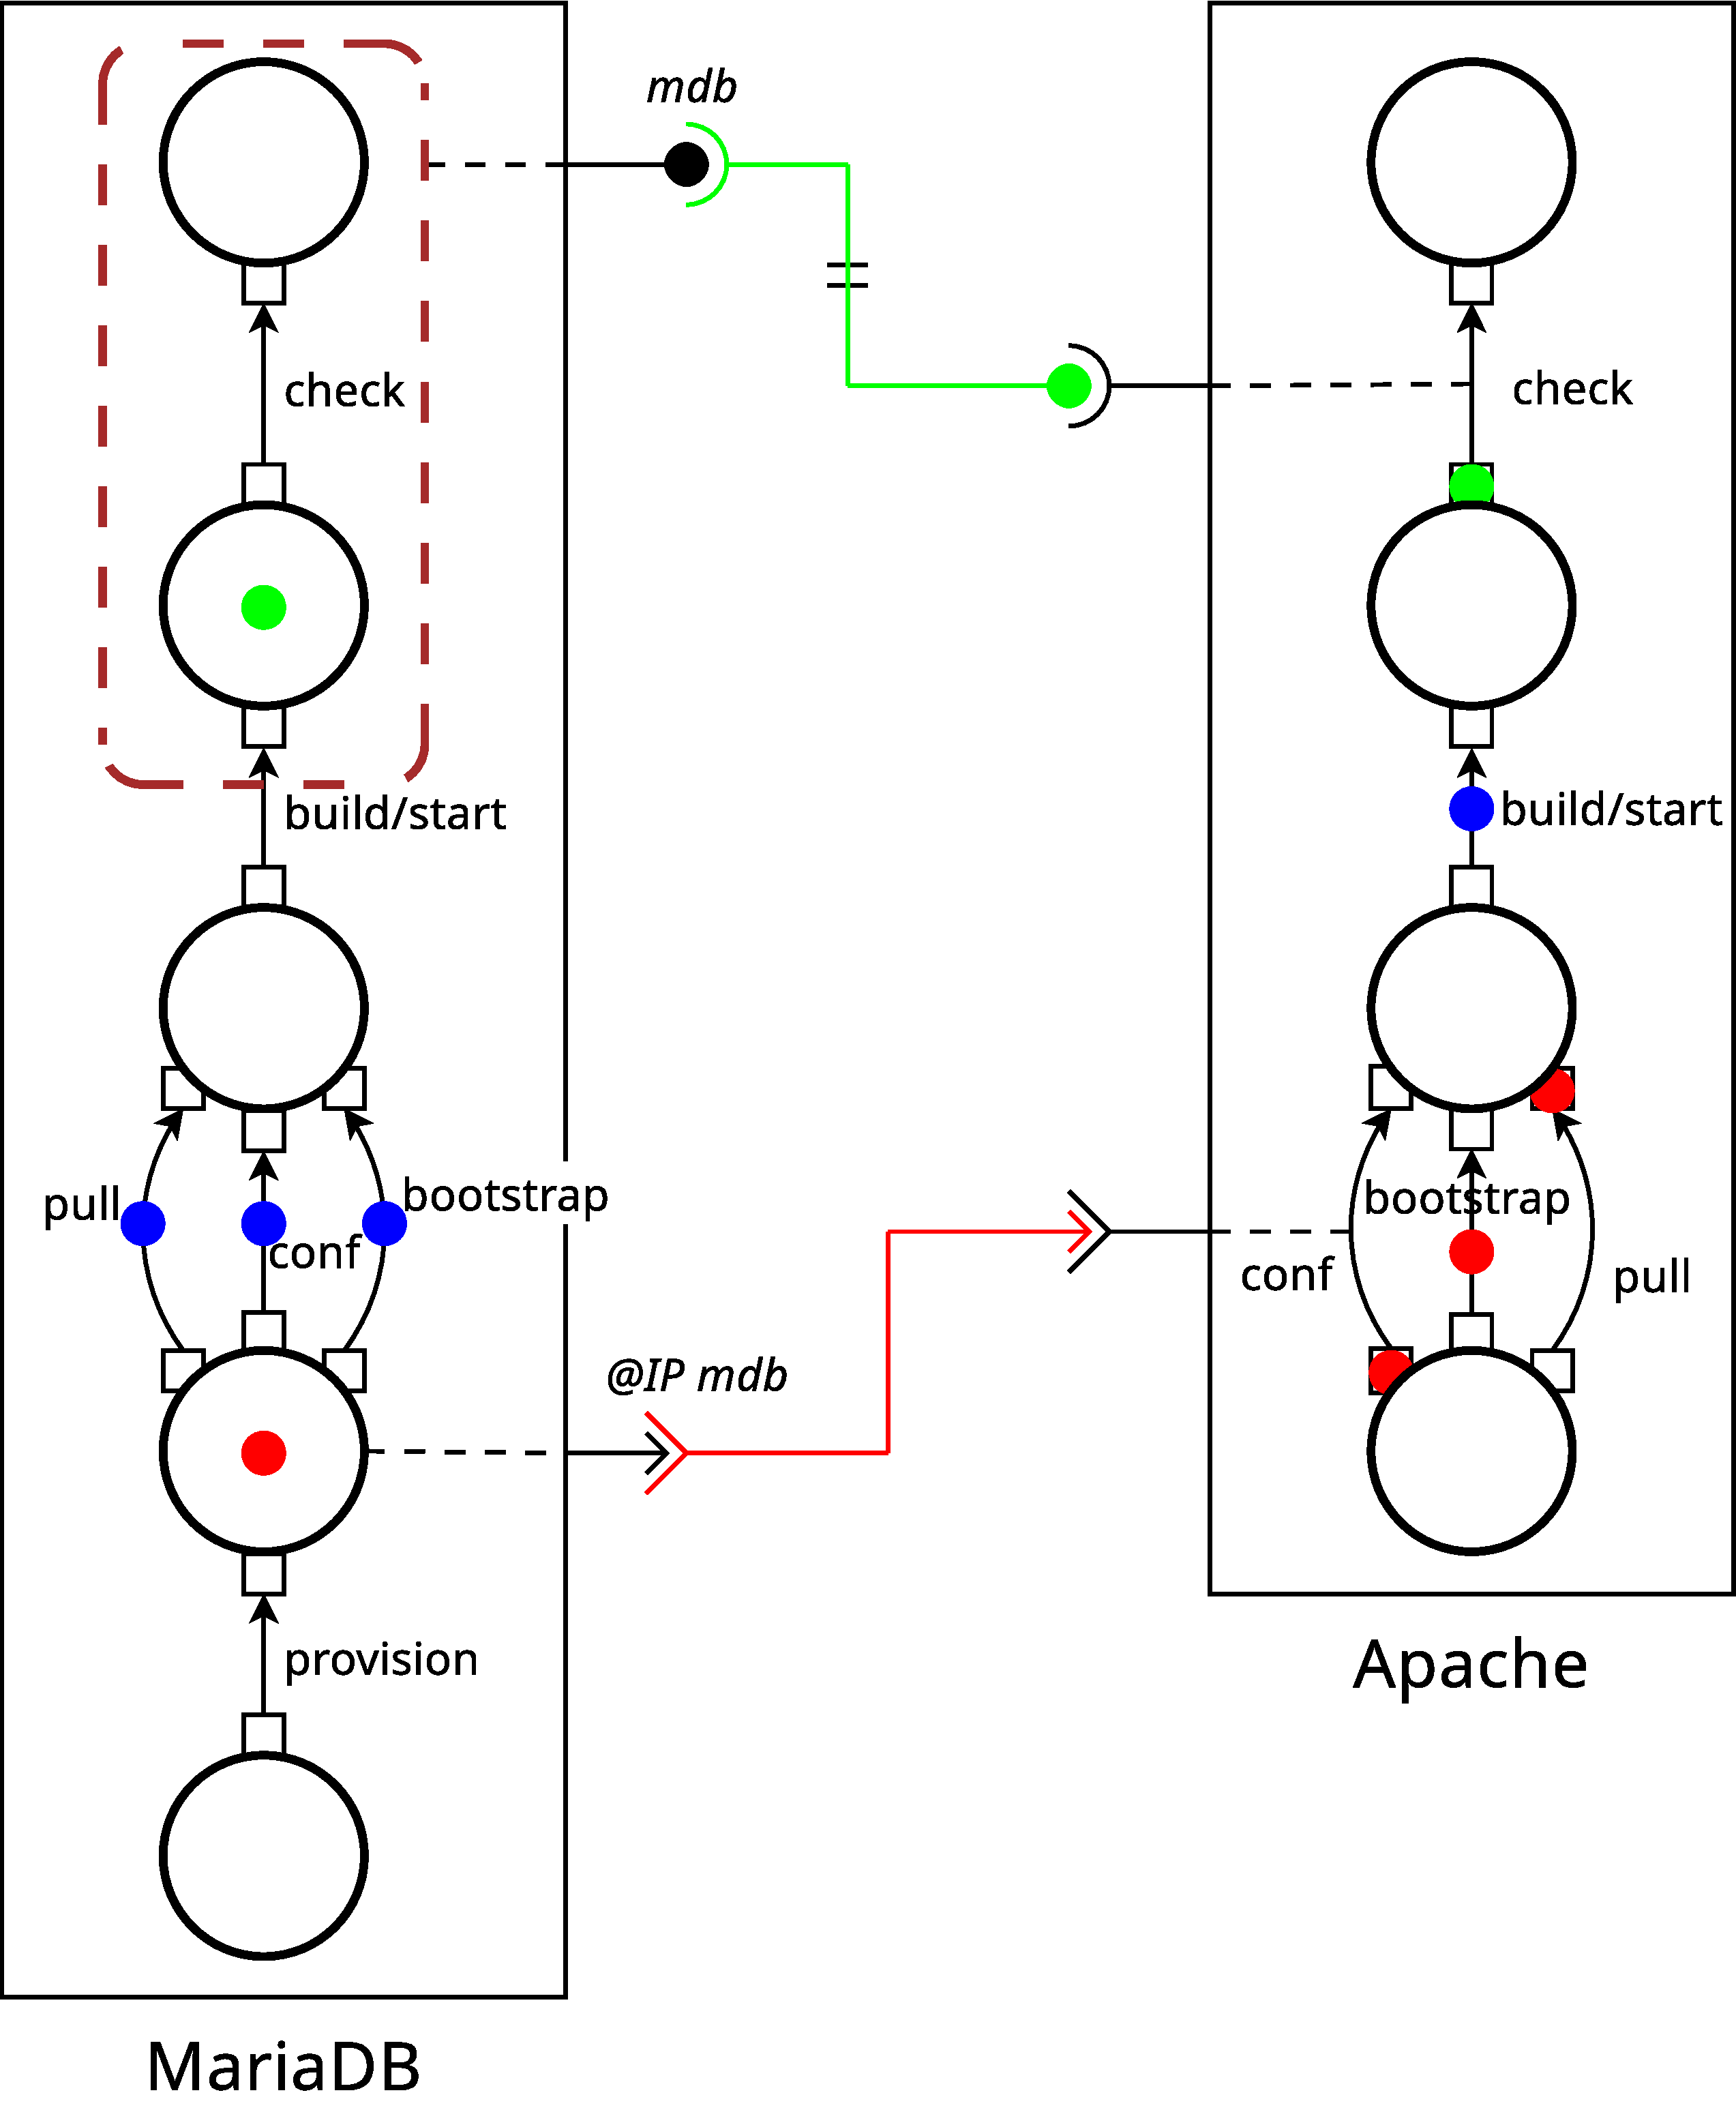
\includegraphics[width=0.7\linewidth]{./images/scenari.pdf}
  \end{center}
  \caption{Three possible intermediate configurations during the commissioning
  of the assembly presented in Figure~\ref{fig:example}. Each configuration is
  represented by a different color.}
  \label{fig:scenari}
\end{figure}

\paragraph{Example}{
We now discuss the commissioning execution of the Apache/MariaDB
example.  The initial assembly, given in Figure~\ref{fig:example}, has
already been described. Figure~\ref{fig:scenari} depicts three example
configurations that may occur at different steps of the
commissioning. In chronological order, the first configuration is
represented by red tokens, the second one by blue tokens, and the
third one by green tokens.

In the first configuration, on the one hand, the red token of MariaDB
has been able to move from its initial place to its output transition
\texttt{provision}, then to execute the action associated to this
transition, to finally reach its second place. One can note that in
this place MariaDB provides data that corresponds to the IP adress
previously got from the \texttt{provision} transition. As soon as this
second place is reached, the associated connection is activated and the
data is considered available. On the other hand, the initial token
of Apache has been duplicated in three tokens, one for each output
dock. Two of these tokens have been able to fire respectively the
transitions \texttt{bootstrap} and \texttt{pull}, and \texttt{pull}
has been ended. However, the third token has remained in its dock,
waiting for the connection bound to the transition \texttt{conf} to be
enabled. In this configuration, as the connection is activated,
the transition \texttt{conf} may be fired.
% SR: ancienne formulation
%the next round of semantics will fire the transition \texttt{conf}.

The blue configuration illustrates a case where parallel transitions
\texttt{pull}, \texttt{conf}, and \texttt{bootstrap} of MariaDB are
executed simultaneously.

Finally, the green configuration illustrates an example where
MariaDB reaches its penultimate place included in the group that
provides a service. As soon as this place holds a token, its
associated provide connection is enabled. As a result, the
\texttt{check} transition of Apache that is using services of MariaDB
can be fired by semantic rules.}
